% Made up for the tikra benchmark.
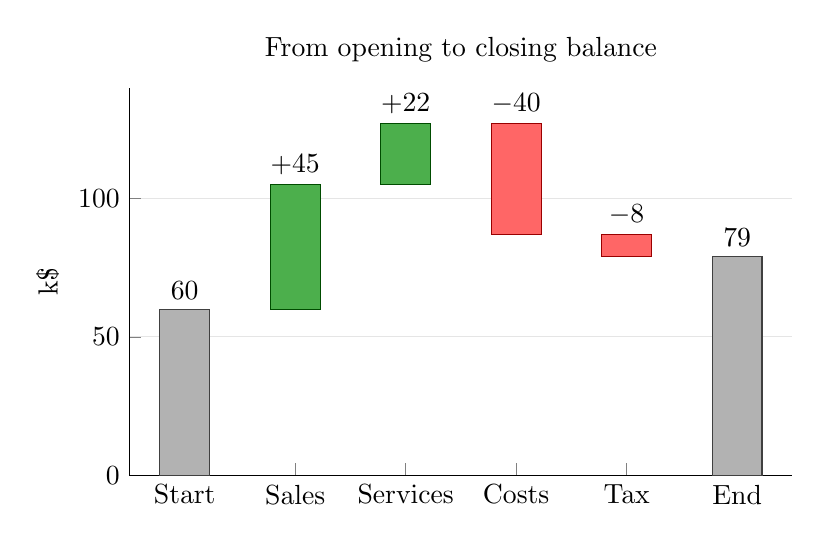
\begin{tikzpicture}
\begin{axis}[ybar stacked, bar width=18pt, width=10cm, height=6.5cm, ymin=0, ymax=140,
    symbolic x coords={Start, Sales, Services, Costs, Tax, End}, xtick=data,
    ylabel={k\$}, title={From opening to closing balance}, ymajorgrids, grid style={gray!20},
    axis x line*=bottom, axis y line*=left, enlarge x limits=0.1]
  % invisible base
  \addplot[draw=none, fill=none, forget plot] coordinates
    {(Start,0) (Sales,60) (Services,105) (Costs,87) (Tax,79) (End,0)};
  \addplot[fill=gray!60, draw=gray!50!black] coordinates
    {(Start,60) (Sales,0) (Services,0) (Costs,0) (Tax,0) (End,79)};
  \addplot[fill=green!55!black!70, draw=green!30!black] coordinates
    {(Start,0) (Sales,45) (Services,22) (Costs,0) (Tax,0) (End,0)};
  \addplot[fill=red!60, draw=red!60!black] coordinates
    {(Start,0) (Sales,0) (Services,0) (Costs,40) (Tax,8) (End,0)};
  \node[above] at (axis cs:Start,60) {60};
  \node[above] at (axis cs:Sales,105) {+45};
  \node[above] at (axis cs:Services,127) {+22};
  \node[above] at (axis cs:Costs,127) {$-40$};
  \node[above] at (axis cs:Tax,87) {$-8$};
  \node[above] at (axis cs:End,79) {79};
\end{axis}
\end{tikzpicture}
